\subsection{Khảo sát theo số luồng}
\label{sec:scaling}
Phiên riêng ngày 25/11 dùng lại đường đi, vòng có cung ngẫu nhiên và phân tầng hoán vị sau khi xác minh SHA-256 của danh sách cung và đối chiếu hồ sơ các tầng. Mỗi đồ thị có 11 cấu hình, gồm Serial một luồng và hai bản OpenMP với $p\in\{1,2,4,8,12\}$, lịch tĩnh. Thứ tự cấu hình xoay giữa các vòng. Phiên hoàn thành 66 lượt khởi động và 396 mẫu chính thức. Mỗi lượt đều được kiểm tra bằng mảng khoảng cách tham chiếu và số luồng thực tế. Mốc Serial được đo cùng phiên.

\begin{figure}[!htbp]
\centering
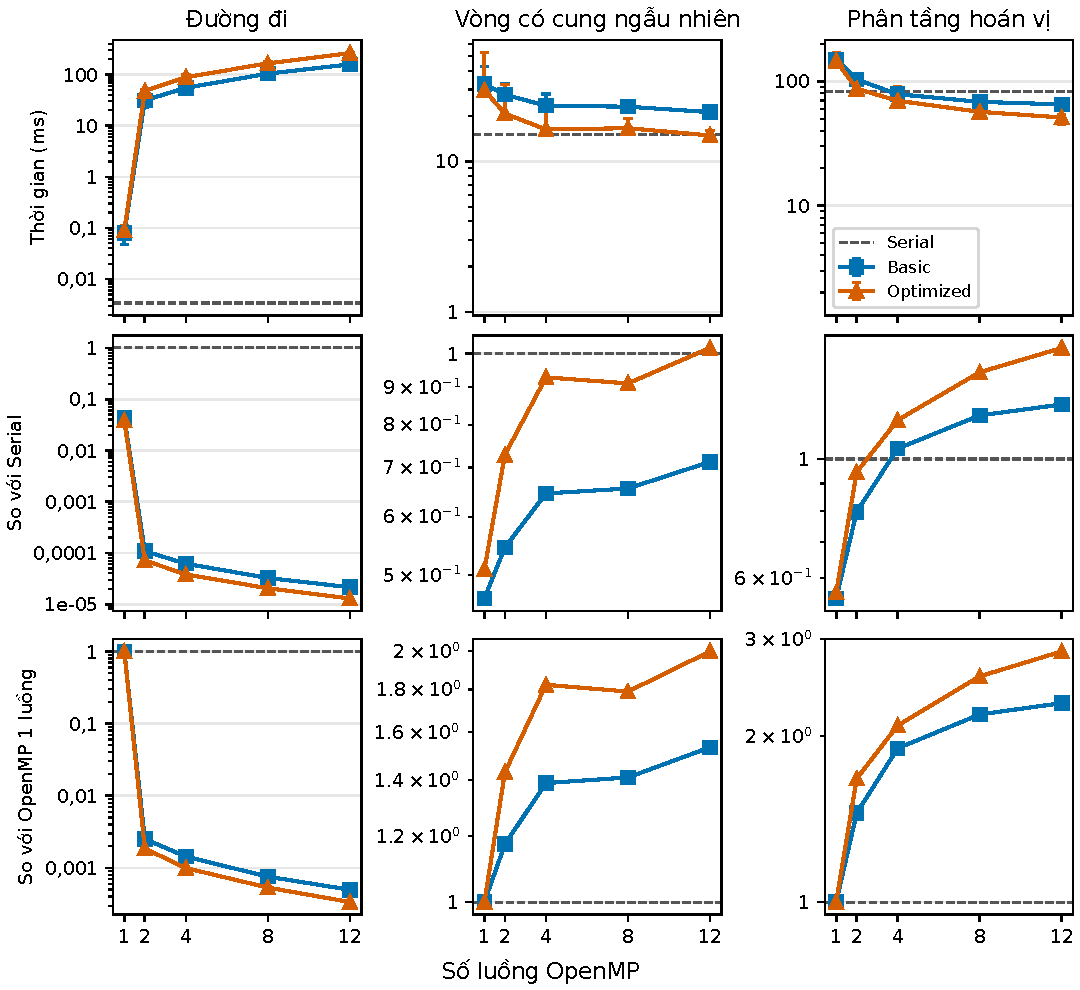
\includegraphics[width=.95\textwidth]{figures/thread-scaling.pdf}
\caption[Thời gian và hệ số theo số luồng]{Phiên khảo sát luồng với 12 mẫu chính thức mỗi cấu hình. Hàng trên là trung vị và khoảng $[Q_1,Q_3]$. Hai hàng dưới lần lượt dùng Serial và OpenMP một luồng làm mốc. Các trục đứng dùng thang logarit.}
\label{fig:scaling}
\end{figure}

Trên đường đi, Serial mất \num{0.0034} ms. Optimized tăng từ \num{0.0887} ms ở một luồng lên \num{166.23} ms ở tám luồng và \num{263.56} ms ở 12 luồng. Hai bản OpenMP đều chậm dần khi tăng số luồng. Kết quả này nhất quán với cấu trúc chỉ có một đỉnh mỗi tầng.

Vòng có cung ngẫu nhiên có trung vị Optimized \num{16.609} ms ở tám luồng và \num{14.863} ms ở 12 luồng, so với Serial \num{15.133} ms. Mức tăng tốc ở 12 luồng xấp xỉ \num{1.02}. Các khoảng tứ phân vị chồng lấn, vì vậy chênh lệch trung vị nhỏ cần được diễn giải thận trọng. Basic có trung vị thấp nhất ở 12 luồng trong các mức của chính Basic, nhưng vẫn chậm hơn Serial.

Phân tầng hoán vị cải thiện từ \num{56.797} ms ở tám luồng xuống \num{51.179} ms ở 12 luồng với Optimized. Ở 12 luồng, hệ số so với Serial là \num{1.61}, hiệu suất là \num{13.4}\%, và hệ số nội bộ so với Optimized một luồng là \num{2.85}. Hình~\ref{fig:scaling} và Phụ lục~\ref{app:scaling} ghi toàn bộ mức luồng. CPU có tám nhân vật lý, 12 luồng logic. Nhóm dùng cách bố trí luồng mặc định của hệ điều hành và runtime, vì vậy dữ liệu chưa cho biết tác động riêng của P-core, E-core hoặc SMT.
